%%%%%%%%%%%%%%%%%%%%%%%%%%%%%%%%%
%
%       EXERCÍCIO
%
%%%%%%%%%%%%%%%%%%%%%%%%%%%%%%%%%

\ifdefstring{\atividade}{prova}{%
    \ifdefstring{\modo}{objetivo}{%
        \renewcommand{\valorquestao}{\ValorQObj\ ponto}
    }{%
        \renewcommand{\valorquestao}{\ValorQDisc\ pontos}
    }%
}%

\begin{exercicioBanco}[\valorquestao]
No diagrama a seguir, \(A, B\) e \(C\) são três conjuntos não vazios.

\begin{center}
    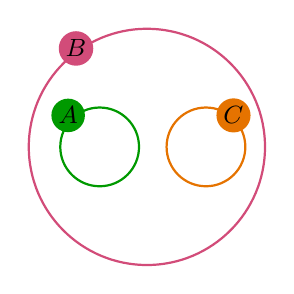
\begin{tikzpicture}[scale=0.5]
        % Conjunto B (maior)
        \draw[thick, purple!70] (0,0) circle (3);

        % Conjunto A
        \draw[thick, green!60!black] (-1.2,0) circle (1);

        % Conjunto C
        \draw[thick, orange!90!black] (1.5,0) circle (1);

        % Rótulos com bolinhas coloridas
        \node[circle, fill=purple!70, text=black, inner sep=1pt] at (-1.8,2.5) {\small$B$};
        \node[circle, fill=green!60!black, text=black, inner sep=1pt] at (-2,0.8) {\small$A$};
        \node[circle, fill=orange!90!black, text=black, inner sep=1pt] at (2.2,0.8) {\small$C$};
    \end{tikzpicture}
\end{center}

Assinale verdadeira (V) ou falso (F) a cada uma das seguintes sentenças.
%
\begin{enumerate}[I.]
    \begin{multicols}{5}
    \item \(A \cap B = \varnothing\).
    %
    \item \(A \subseteq B\).
    %
    \item \(\varnothing \subseteq A\).
    %
    \item \(A \cup C = B\).
    %
    \item \(B\setminus A = C\).
    \end{multicols}
\end{enumerate}

% Define as alternativas
\newcommand{\alternativas}{%
    \begin{center}
        \begin{tabularx}{\textwidth}{XXXXX}
            (a) (F, V, F, V, V). &
            (b) (V, V, V, F, F). &
            (c) (F, V, F, V, F). &
            (d) (V, F, V, F, F). &
            (e) (V, F, V, F, V).
        \end{tabularx}
    \end{center}
}

% Define a resposta correta
\newcommand{\resposta}{B}

% Lógica condicional para exibição
\ifdefstring{\atividade}{lista}{%
    \alternativas
    \vspace{0.5em}
    
    \noindent\textbf{Resposta:} letra \textbf{\resposta}.
}{%
    \ifdefstring{\modo}{objetivo}{%
        \alternativas
    }{%
        % modo = discursiva → não mostra alternativas
    }
}
\end{exercicioBanco}

